\documentclass[10pt]{article}

\usepackage{fullpage}
\usepackage{graphicx}
\usepackage{mathtools}
\usepackage{setspace}
\usepackage{mdwlist}
\usepackage[center,font=singlespacing]{caption}
\usepackage{subfig}
\usepackage{hyperref}
\onehalfspacing
\usepackage{listings}	  	
\usepackage{verbatim}

\begin{document}
\lstset{language=Verilog,numbers=left, numberstyle=\tiny, stepnumber=2, numbersep=5pt,basicstyle=\small,frame=Tl,breaklines=true,breakautoindent=true}	
\title{Recursive Augmented Reality Image Processing System}
\author{Logan P. Williams \& Jos\'{e} E. Cruz Serrall\'{e}s}
\date{December 10, 2011}
\maketitle

\section*{Abstract}
We have implemented an augmented reality system that can overlay a digital image on video of a real world environment. We read NTSC video from a video camera and store it in ZBT memory. A picture frame with colored markers on the corners is held in front of the camera. We then perform chroma-based object recognition to locate the coordinates of the corners. Using these coordinates, we apply a projective transformation to project an image onto the dimensions of the picture frame. We then output VGA video of the original captured image, with the processed image overlayed on top of the frame. By using the previously displayed video frame as the image to be projected, the system becomes ``recursive.''

\newpage

\tableofcontents
\listoffigures

\newpage

\section{Overview}
% needs non-technical overview of project goals/motivations/methods

The augmented reality image processing system, or {\tt augreal}, was inspired by the recursive feedback effects created by pointing a video source at its own display. Unfortunately, in doing this in the real world, there is significant loss in image quality in each successive generation. Performing the same operation in digital logic provided the opportunity to achieve the same effect, in real time at a high frame rate, with minimal image quality loss. We also chose to implement object tracking functionality, to simulate the effect of moving the video monitor around within the camera's field of view. The final output of {\tt augreal} is shown in Figure 1.

\begin{figure}[h!]
\centering
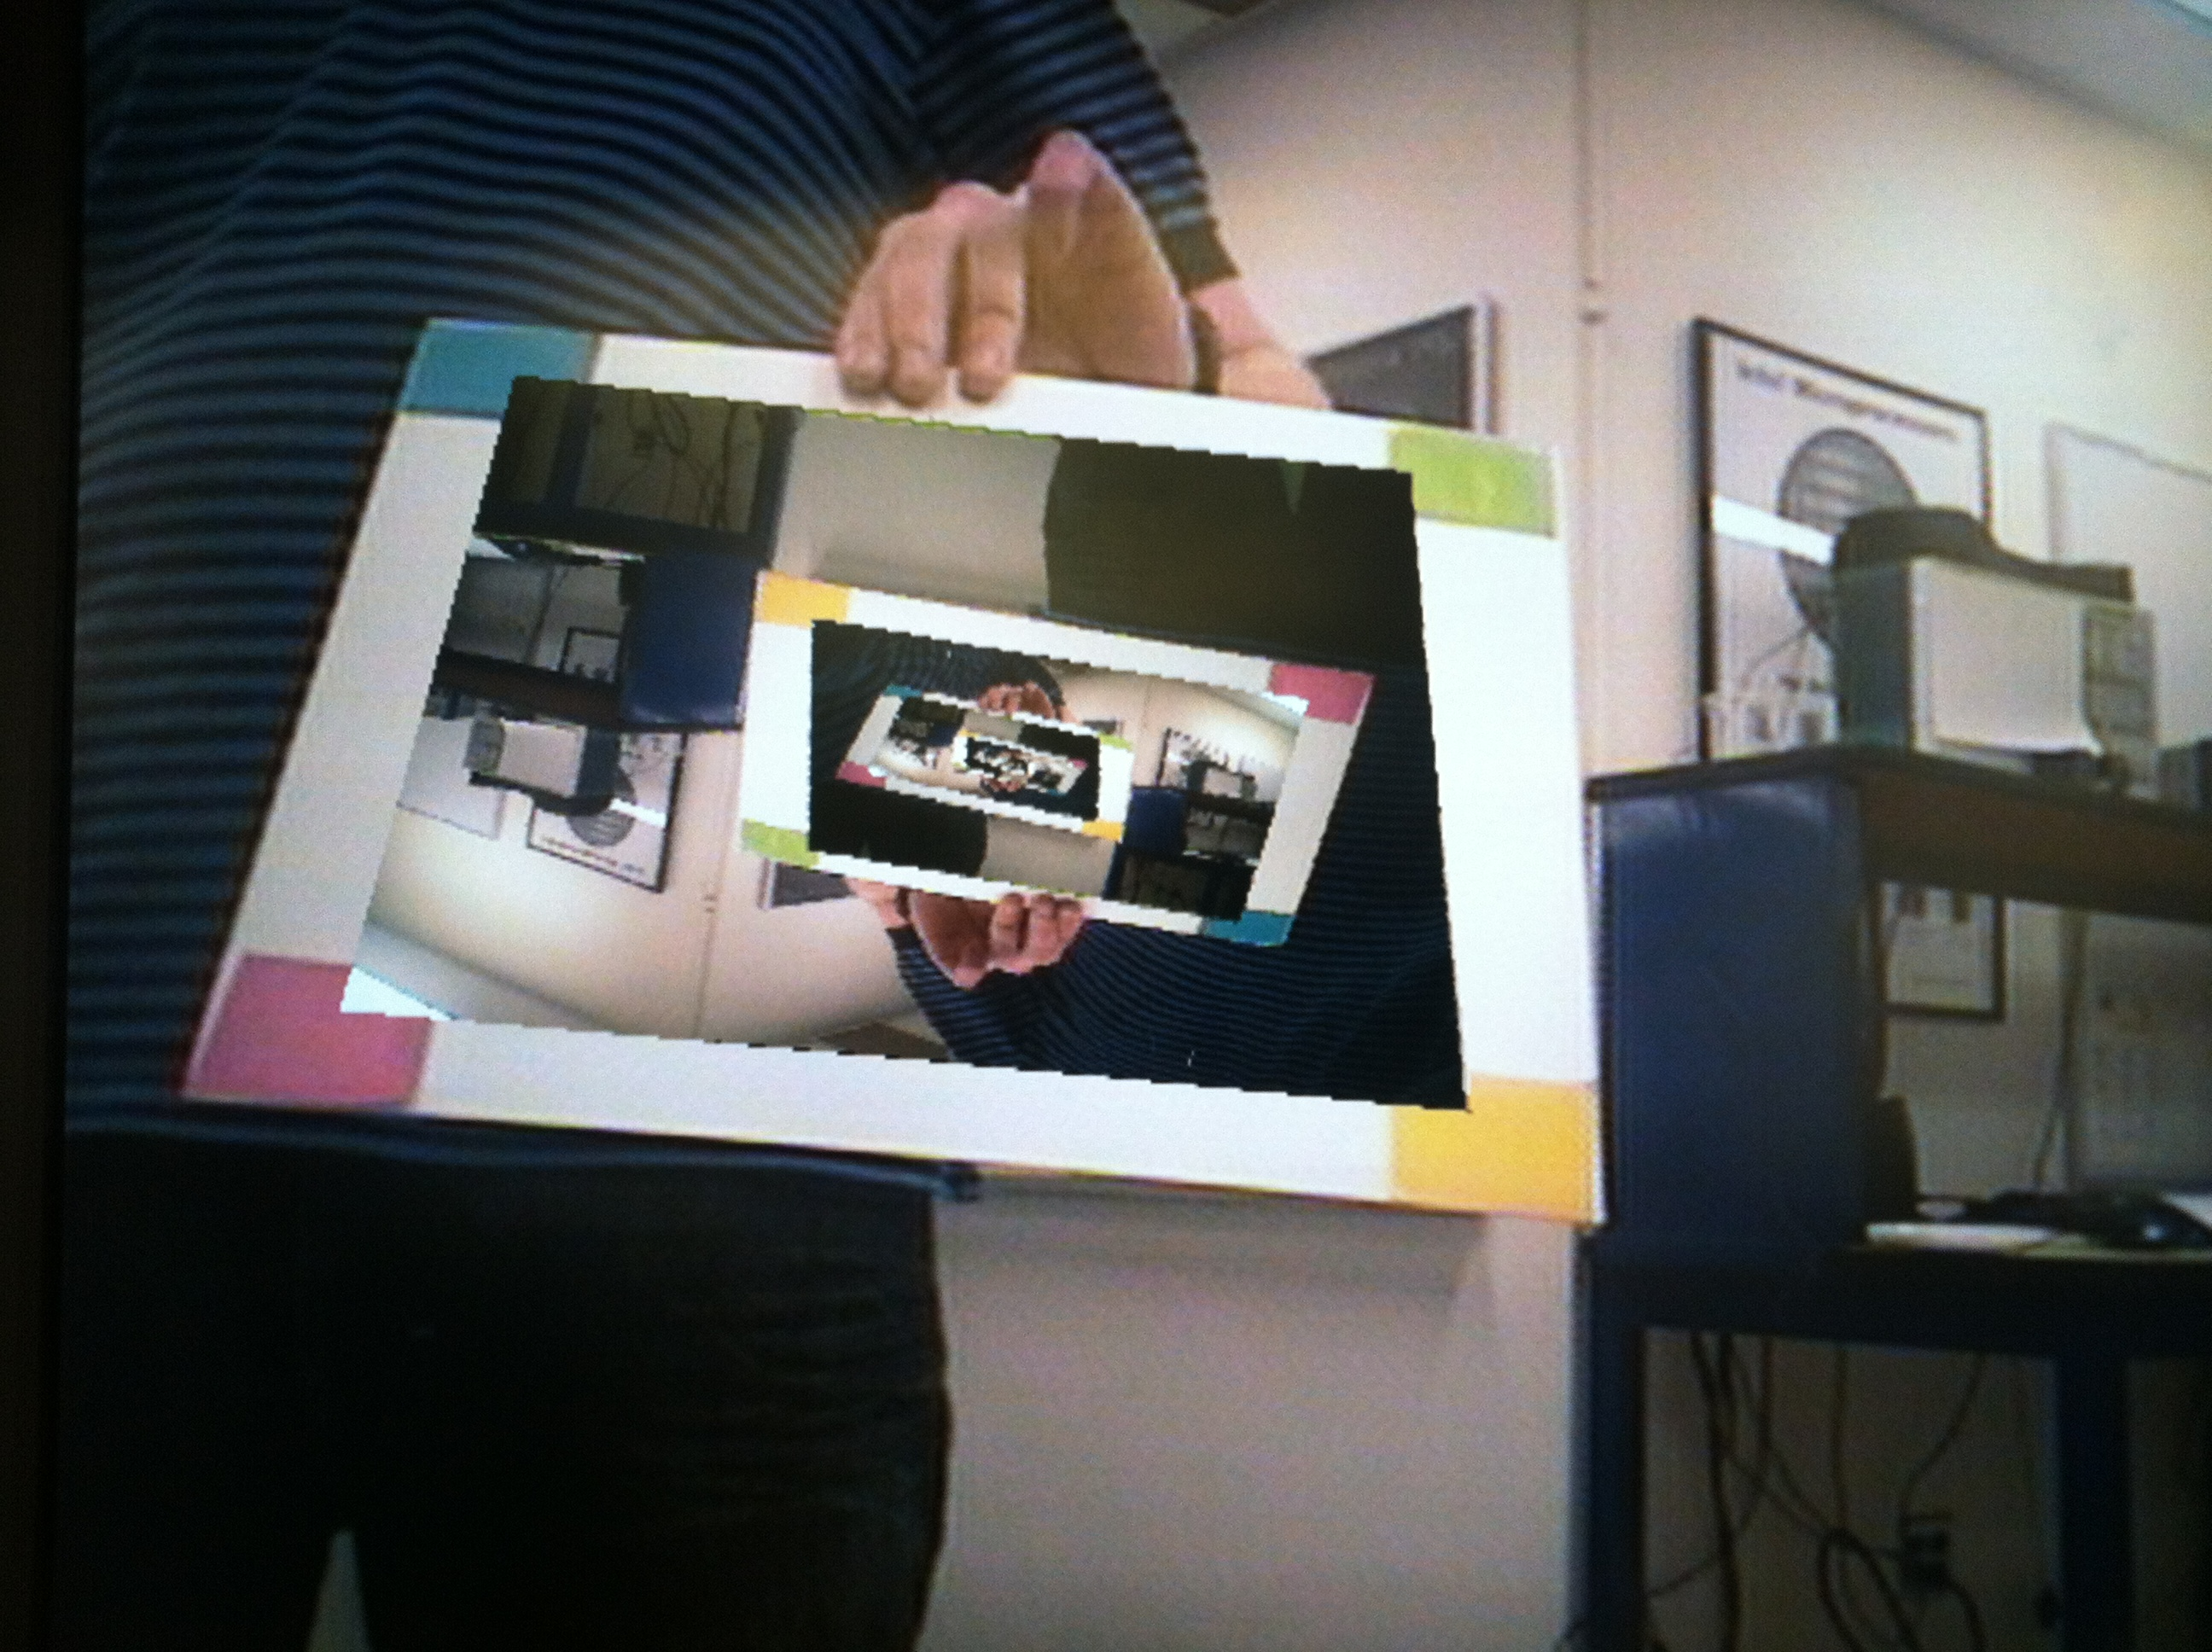
\includegraphics[width=0.75\textwidth]{images/IMG_0113.JPG}
\caption{\emph{A screen capture of the video output of the augmented reality image processing system.}}
\end{figure}

The {\tt augreal} system uses a four stage buffered image processing pipeline. Images from a video camera are captured into a memory buffer, which on the next frame, is partially overwritten by skewed, scaled, and rotated pixels from the last image buffer that was displayed on the VGA output. On the next frame, this overwritten buffer becomes the video output. There are seven primary modules of this system.

The {\tt clock\_gen} module is responsible for creating and phase synchronizing the clocks used by the rest of the system. Because we require a specific video clock frequency, and the amount of computation and memory accesses we must perform, it is necessary for {\tt augreal} to use three distinct clock domains: a video capture clock, at approximately 27 mhz, generated externally by the video camera, a memory clock at 50 mhz, and a video output clock at 25 mhz.

The {\tt memory\_interface} module handles reading and writing from the ZBT memory, abstracting these operations away from the other modules. This module is responsible for ``shifting'' the buffers as described above.

Raw video is read from the video camera by the {\tt ntsc\_capture} module, which also finds recognizes pixels that match the colors of the corners of the target frame. These pixels are read by the {\tt object\_recognition} module which finds the weighted center of mass of the frame corners. The {\tt LPF} module sends each pixel to the {\tt projective\_transform} module which then sends that pixel's value and new coordinates to the {\tt memory\_interface} module to be written to memory. The {\tt vga\_write} module reads and transmits the VGA data to be generated by the video DAC.

Raw video is read from the video camera by the {\tt ntsc\_capture} module, which also finds recognizes pixels that match the colors of the corners of the target frame. These pixels are read by the {\tt object\_recognition} module which finds the weighted center of mass of the frame corners. The {\tt LPF} module sends each pixel to the {\tt projective\_transform} module which then sends that pixel's value and new coordinates to the {\tt memory\_interface} module to be written to memory. The {\tt vga\_write} module reads and transmits the VGA data to be generated by the video DAC.

\begin{figure}[h!]
\centering
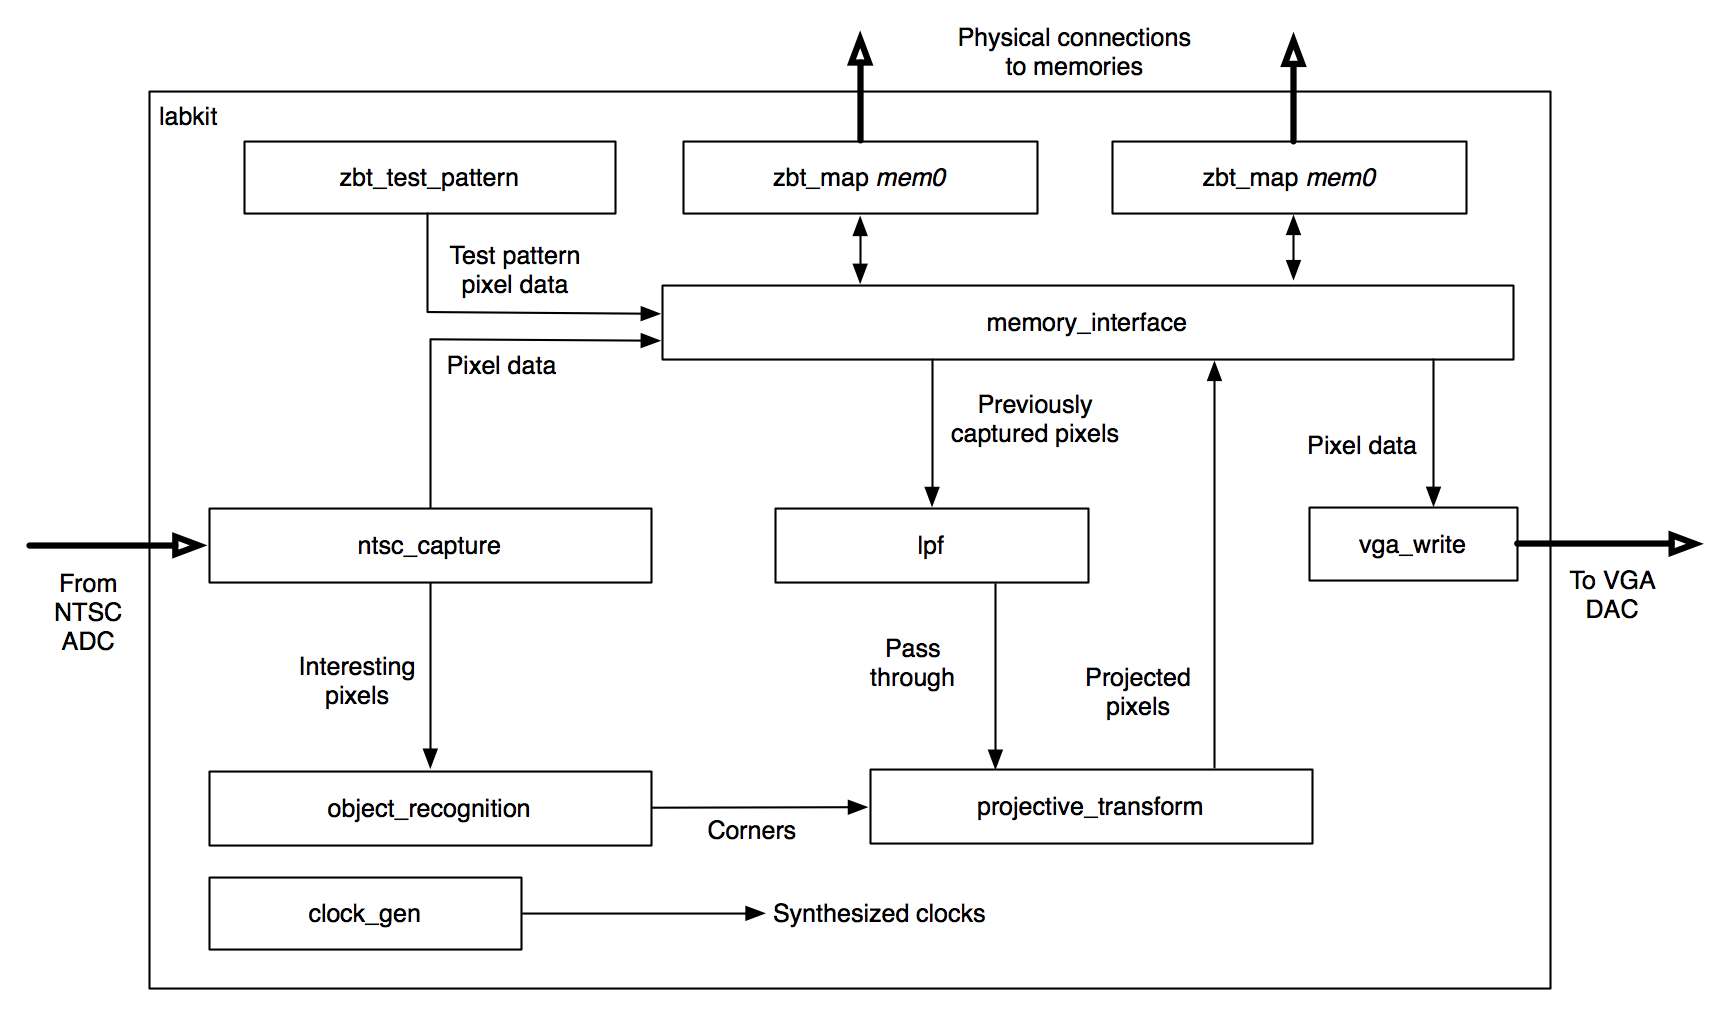
\includegraphics[width=\textwidth]{images/simplified_block_diagram.png}
\caption{\emph{An overview block diagram of the augmented reality system.}}
\end{figure}

\section{Description}

\subsection{{\tt ntsc\_capture} (Logan)}
The {\tt ntsc\_capture} module decodes NTSC Composite video using an Analog Devices ADV7185 video ADC and sends pixels in luminance/chrominance color space to {\tt memory\_interface} to be written into a ZBT memory frame buffer. Additionally, {\tt ntsc\_capture} is responsible for recognizing colors that matches the corner targets (blue, green, pink, and orange).

{\tt ntsc\_capture} has three submodules, none of which were written by our team. They are described here with specific attention to their relation to the primary {\tt ntsc\_capture} module.

\paragraph{{\tt adv7185init}} This module initializes the ADV7185 video ADC. It selects the video source (in our case, the composite video input), and wires the data streams to the {\tt labkit} module. This module was written by the 6.111 staff.

\paragraph{{\tt ntsc\_decode}} This module takes the incoming data stream from the ADV7185, and decodes it into individual pixels. It also generates flags that indicate when its data output is valid, when the NTSC stream is in horizontal sync, when the NTSC stream is in vertical sync, and whether the current frame is an odd or even field. (Because NTSC video data is interlaced, each frame alternates even and odd lines of video.) This module was written by the 6.111 staff.

\paragraph{{\tt ntf}} The {\tt ntsc\_capture} module generates data at the speed of the external video clock, which is ~27 Mhz. This creates problems with processing that data in modules that operate at the RAM clock speed of 50 Mhz. To solve this problem, {\tt ntf} is a dual clock domain FIFO register, generated by the Xilinx Core Generator utility. Data is written to it on the video clock domain, and read from it on the RAM clock domain. In this way, flags and pixels are synchronized correctly before being processed by {\tt memory\_interface}.

\paragraph{} {\tt ntsc\_capture} itself uses x and y iterator registers to tell {\tt memory\_interface} where to write the incoming pixels to. The x iterator variable increments every time the data valid output of {\tt ntsc\_decode} goes high. When x is even, the incoming pixel is stored in a buffer, and when it is odd, both the incoming pixel and the previously buffered pixel are sent to {\tt memory\_interface}. When a horizontal sync is detected, the y iterator variable increments by two, because of the interlacing of the video stream. When a vertical sync is detected, the x iterator variable resets to 0, but the y iterator variable resets to  the current field value, in order to ``seed'' the y iterator as even or odd. {\tt ntsc\_capture} ignores the first 23 lines of video input, and the first 10 pixels of each line, as it was found in testing that those pixels are always blanked.

In both states, comparisons are also made with threshold parameters in luminance and chrominance to check for ``interesting'' colors, and when detected, a flag and the color detected are sent to {\tt object\_recognition} through the {\tt ntf} FIFO memory. The threshold values for detection can be adjusted using the buttons on the labkit. These values are generated and stored by the {\tt parameter\_set} module.

\subsection{{\tt memory\_interface} (Jos\'{e})}
% Jose
The {\tt memory\_interface} module handles the interactions between all of the other modules and the two ZBT Memory blocks, which house the four images that the modules use for capturing, displaying, and processing. Ideally, BRAM would have been used, but the number of pixels that we would like to store vastly exceeds BRAM capacity. Unlike BRAM, each ZBT Memory block can only handle one read or write operation per cycle, causing memory access to be the main bottleneck of our system. As such, we store only 8 bits of luminance and 5 bits of each chrominance per pixel, allowing us to store two pixels per address and to reduce the number of memory accesses in our system by a factor of two. The number of required memory acceses per module and the distribution of the images in the RAM necessitates a minimum clock frequency of 35MHz.

The inputs to {\tt memory\_interface} are (1) {\tt frame\_flag}, which signals when to shift; (2) {\tt ntsc\_pixel}, the two pixels from {\tt ntsc\_capture}; (3) four (x,y) pairs; (4) one pixel from {\tt projective\_transform}; and (5) request flags. The outputs from {\tt memory\_interface} are (1) done flags; (2) a pixel pair to {\tt vga\_write}; and (3) two pixels to {\tt LPF}.

{\tt memory\_interface} allocates two images per memory block. These four images are (1) {\it capture}, the image being captured from NTSC; (2) {\it display}, the image being displayed in the VGA; (3) {\it processing}, the image that is processed by {\tt LPF}; and (4) {\it next\_display}, the image to which {\tt projective\_transform} writes and the next image that will be displayed. Every image refresh (1/30 seconds), the previous {\it next\_display}, {\it display}, {\it capture}, and {\it processing} image locations become the next {\it display}, {\it processing}, {\it next\_display}, and {\it capture} image locations, respectively. These location shifts are transparent to the other modules. Read and write requests from {\tt vga\_write} and {\tt ntsc\_capture} will be given priority over requests from other modules.

\begin{figure}[h!]
\centering
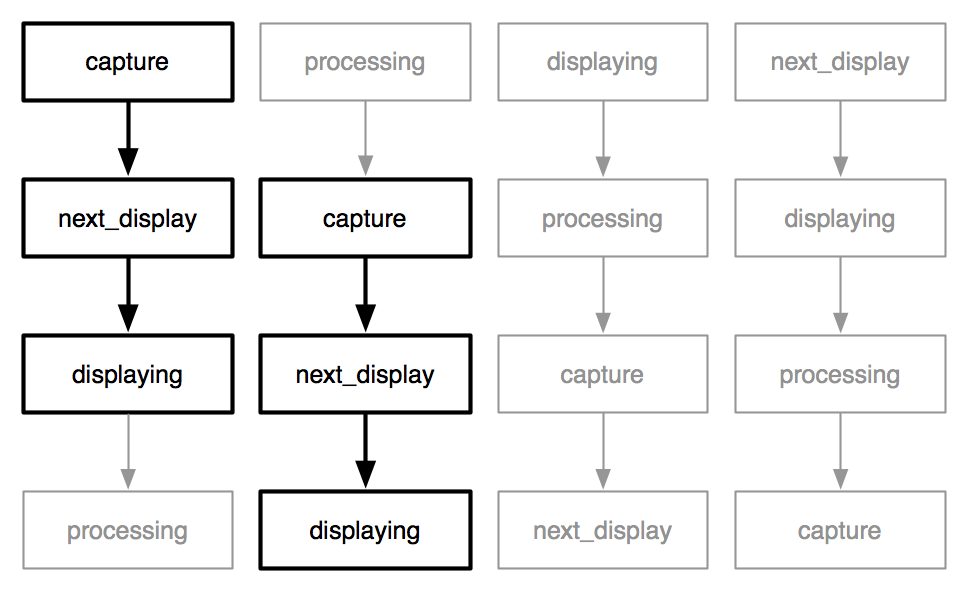
\includegraphics[width=0.75\textwidth]{images/buffers.png}
\caption{{\emph The progression seen in memory locations as {\tt frame\_flag} is asserted. Two complete pathways from image capture to image display are highlighted.}}
\end{figure}

Due to the two-cycle latency of the ZBT RAM, care was taken in {\tt memory\_interface} to wait two cycles before assigning an output to the module that made a request. Additionally, {\tt zbt\_map} was used to delay the write data to the RAM by two cycles. Additionally, {\tt zbt\_map} allows for {\tt memory\_interface} to request partial bit write enables, which proved to be necessary for the operation of {\tt projective\_transform}. {zbt\_map} was adapted from the {\tt zbt\_6111} module.

\subsection{{\tt object\_recognition} (Logan)}
The {\tt object\_recognition} module collects ``interesting'' pixels located by the NTSC Capture module, and calculates the center of mass of each color, to find the location of the corners of the picture frame.

It takes as inputs (1) the color of a detected pixel, (2) a flag that goes high for one clock cycle when a pixel is detected, (3) the X/Y coordinates of the pixel, and (4) a flag that goes high when a new frame is beginning. It produces as output four sets of X/Y coordinates, one for the center of mass of each color.

Instead of performing a linear average of interesting pixels recieved in each color, we chose to implemented a weighted average, in order to make the module more resistant to noise and interference from background objects. When {\tt object\_recognition} recieves a flag from {\tt ntsc\_capture}, it multiplies that pixel's coordinates proportionally to their distance from the center of mass generated in the last frame. These modified coordinates are accumulated in seperate registers for each color. Upon receipt of a {\tt frame\_flag}, the module initializes the divide operation to perform the averaging. (The functionality of the {\tt divider} submodule is described in detail in the {\tt projective\_transform} section below.)

After the completion of this division operation, the {\tt object\_recognition} module calculates the minimum side length in the horizontal and vertical direction. These distances were intended to be used by {\tt lpf} for generating downsampling coefficients, but this functionality was not implemented.

\subsection{{\tt LPF} (Jos\'{e})}
The warping of images carried out by {\tt projective\_transform} aliases the image, resulting in undesired ``junk'' pixels. Initially, {\tt LPF} was thought up as a way to lowpass the pixel data and avoid aliasing. Unfortunately, due to time constraints and unforeseen, extensive issues in getting video capture, memory interfacing, and video display to work, an {\tt LPF} module that lowpasses pixel data was not written. Instead a simple {\tt LPF} was written that fetches pixels from memory when {\tt projective\_transform}'s {\tt request} is asserted high, and four cycles later, pulses {\tt pixel\_flag} and outputs one pixel. {\tt LPF} pulses its {\tt lpf\_flag} once every two pixels, that is, only on even pixel requests.

The inputs to {\tt LPF} are (1) {\tt frame\_flag}, which indicates the start of a new cycle; (2) {\tt done\_lpf}, which indicates that the module's memory request was processed; (3) {\tt lpf\_pixel\_read}, the pixels from {\tt memory\_interface}; and (4) {\tt request} from {projective\_transform}. The outputs from {\tt LPF} to {\tt memory\_interface} are (1) {\tt lpf\_flag}, and (2) {\tt lpf\_x} and {lpf\_y}, the (x,y) coordinates of the leftmost pixel. The outputs from {\tt LPF} to {\tt projective\_transform} are (1) {\tt pixel\_flag}, which signals when a new pixel is available, and (2) {\tt pixel}.

The intended operation of {\tt LPF} was to apply a lowpass filter (LPF) to the {\it processing} image so as to avoid aliasing when {\tt projective\_transform} skews the image. The following steps detail the procedure that would have been carried out by {\tt LPF} every image refresh cycle (1/30 seconds): (1) Load the filter coefficients of a 1D LPF with cutoff frequency \( \frac{\pi}{M_y} \). (2) Apply this filter to each column of {\it processing} and store each column once again in {\it processing}. (3) Load the filter coefficients of a 1D LPF with cutoff frequency \( \frac{\pi}{M_x} \). (4) Apply this filter to each row of {\it processing} but instead feed the output pixels to {\tt projective\_transform}. (5) Wait for the next cycle. The image data will be buffered in BRAM, such that LPF accesses memory 1.5 times per pixel.

The lowpass filters that would have been used would have been finite impulse response (FIR) Parks-McClellan filters. Most of the information contained in an image is contained in its phase. FIR filters were chosen because they can be made so as to have no effect on the phase of the image, preserving most of the information. Parks-McClellan filters were chosen because they are highly adaptable and easily calculated with MATLAB. The filter coefficients would have been stored in BRAM for easy access. Because {\tt FIR} will only be filtering the luminance component of each pixel, the order, \( N \), of these filters would have been constrained by the number of multipliers on the FPGA and the number of multipliers used in other modules. The symmetry of these filters would have been exploited, requiring only \( \frac{N}{2}+1 \) multiplications per pixel.

\subsection{{\tt projective\_transform} (Logan)}
% Logan
The inputs to {\tt projective\_transform} are (1) the pixel value last produced by {\tt LPF}, (2) a flag signal held high for one clock signal when {\tt LPF} has processed a new pixel, (3) the four coordinates of the corners of the frame provided by the {\tt object\_recognition} module, and (4) a signal when a new frame is beginning.

The outputs from {\tt projective\_transform} are (1) a request to {\tt LPF} for a new pixel, (2) the X/Y coordinates of the transformed pixel, (3) the transformed pixel value, and (4) a flag indicating that a new pixel is to be written.

This function maps the original rectangular image to any convex quadrilateral, provided that all sides of the destination quadrilateral are shorter than the original, which is inherent in the overall system. A graphic representation of the transformation is shown in Figure 2.

\begin{figure}[h!]
\centering
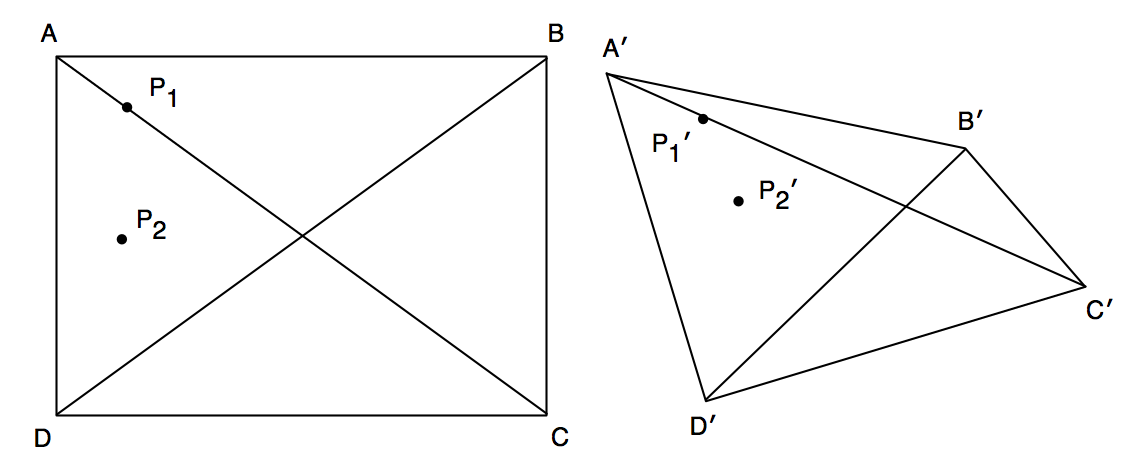
\includegraphics[width=0.85\textwidth]{images/arbiskew_graphic.png}
\caption{\emph{A visual representation of the result of the {\tt projective\_transform} module. Input is on the left, a possible output, for four coordinates $A\prime$, $B\prime$, $C\prime$, and $D\prime$ is on the right.}}
\end{figure}

Mathematically, the algorithm works as follows:
\begin{enumerate*}
\item Create two ``iterator points,'' point $I_A$ and $I_B$ initially located at $A\prime$ and $B\prime$.
\item Create a third iterator point, $I_C$ at the location $I_A$.
\item Let $o_x = 0$ and $o_y = 0$

\item Calculate the normalized incrementor value, {\tt delta\_a\_x} $= \Delta_{ax}/480$.
\item Calculate the normalized incrementor value, {\tt delta\_a\_y} $= \Delta_{ay}/480$.
\item Repeat steps 1 and 2 for {\tt delta\_b\_x} and {\tt delta\_b\_y}.
\item Calculate the normalized incrementor value, {\tt delta\_c\_x} $= \Delta_{cx}/640$.
\item Calculate the normalized incrementor value, {\tt delta\_c\_y} $= \Delta_{cy}/640$.

\item Assign the pixel value of $I_C$ to pixel $(o_x, o_y)$ in the original image.
\item Increment the coordinate of $I_C$ by ({\tt delta\_c\_x}, {\tt delta\_c\_y}).
\item Increment $o_x$.
\item Repeat steps 9--11 until $I_C = I_B$.

\item Increment the coordinate of $I_A$ by ({\tt delta\_a\_x}, {\tt delta\_a\_y}).
\item Increment the coordinate of $I_B$ by ({\tt delta\_b\_x}, {\tt delta\_b\_y}).
\item Increment $o_y$.
\item Repeat steps 7--15 until $I_A = D\prime$ and $I_B = C\prime$.

\end{enumerate*}

The Verilog implementation of this module has two types of submodules. The algorithm requires no multiplications, but several divisions. To perform divisions, a divider module, named {\tt divider}, was used that implemented a simple restoring division algorithm. \cite{restoring} This algorithm takes $N$ clock cycles to complete, where $N$ is the width of the dividend and divisor.

The {\tt LPF} module, which sends pixel data to the {\tt projective\_transform} module, has a five clock cycle delay on transmitted pixels. Because of this, up to five pixels can arrive at {\tt projective\_transform} while it is unable to write to memory, even after {\tt pt} has told {\tt lpf} to stop sending new data. Because of this, it was necessary to create a buffer to hold pixel data until it was able to be written to {\tt memory\_interface}. The {\tt shift18} module accomplishes this by using 18 {\tt SRL16E} 16 bit shift register primitive elements to a create an 18 bit wide shift register. By setting the address of the multiplexer associated with each {\tt SRL16E} element, the length of the shift register can be expanded and contracted easily.

\begin{figure}[h!]
\centering
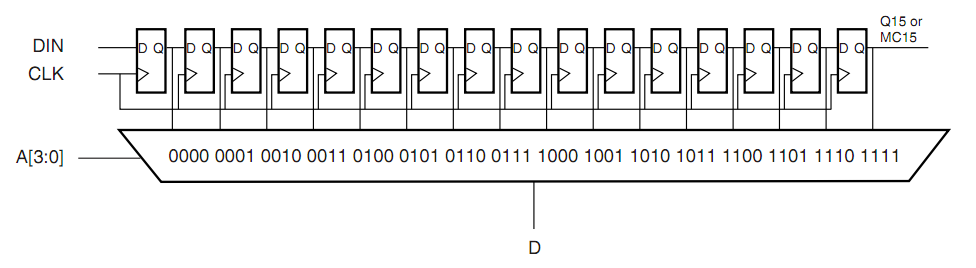
\includegraphics[width=\textwidth]{images/srl16.png}
\caption{\emph{The {\tt SRL16E} primitive shift register element. By setting {\tt A[3:0]}, the length of the buffer can be adjusted dynamically.}}
\end{figure}

The {\tt projective\_transform} module itself is a state machine with three states, {\tt WAIT\_FOR\_CORNERS}, {\tt WAIT\_FOR\_DIVIDERS}, and {\tt WAIT\_FOR\_PIXEL}. The module initializes itself to the {\tt WAIT\_FOR\_CORNERS} state, where it stays until {\tt object\_recognition} indicates with {\tt corners\_flag} that it has finished calculating the location of the four corners of the frame in the image. When this flag is recieved, it initializes the divisors and dividends of each of the six dividers, and sends a signal for the dividers to begin their operation. Then, the machine advances to the {\tt WAIT\_FOR\_DIVIDERS} state.

In this state, the module waits until all of the dividers have finished their computation. When this occurs, the results of each computation are saved in the delta registers. This corresponds to steps 4--6, and the first iteration of 7--8 in the algorithm outlin above. Then the module advances to the {\tt WAIT\_FOR\_PIXEL} state, where the bulk of the algorithm, steps 7--15, is implemented.

In this state, for every clock cycle in which {\tt memory\_interface} indicates that it can accept new data, {\tt projective\_transform} outputs a pixel and a coordinate from its buffer. If {\tt memory\_interface} cannot accept new data (because of a conflict with {\tt ntsc\_catpure} or {\tt vga\_display}, the module tells {\tt lpf} to stop sending new data. If {\tt projective\_transform} receives a new pixel from {\tt lpf}, it buffers it into {\tt shift18}. When $o_x = 500$, {\tt projective\_transform} begins the division operators in steps 7 and 8 for the next line of the image. In this way, the divisions are pipelined so that there is no delay due to {\tt divider}. Without this pipelining, there would be a 42 cycle delay at the beginning of each line of output. When {\tt projective\_transform} has iterated through the complete original image, it resets its iterator variables and its to {\tt WAIT\_FOR\_CORNERS}.

\subsubsection{{\tt clock\_gen (Jos\'{e})}}
Clock synthesis is carried out by this module. Initially, we assumed that clocking would not be much of an issue. However, as we initially tested our modules, we realized that improper clock generation created persistent and pervasive setup and hold time issues. After much trial and error, we settled on using a DCM to generate a reference clock at 50MHz, using this clock to generate the {\tt ram\_clock}s and the system clock, and using the {\tt CLKDV} output to obtain a clock at half the frequency of the system clock. The DCM that synthesizes the system clocks and RAM clocks is located in the {\tt ramclock} module, which is an adapted version of the module provided to us by the staff. In the output DCM of {\tt ramclock}, the parameter {\tt CLKDV\_DIVIDE} had to be set to 2, the parameter {\tt CLKOUT\_PHASE\_SHIFT} was changed to "FIXED", and the parameter {\tt PHASE\_SHIFT} was set to 0. Setting these parameters to their respective values provided us consistent locking.

25MHz was chosen as our video display frequency because it is close to the required 25.175MHz frequency for 640x480x60Hz display. 50MHz was chosen as our system frequency because it met our minimal frequency requirement and because 0-phase locking with the 25MHz signal could be achieved, as 50MHz is an even multiple of 25MHz. This simplified considerably the design of the {\tt vga\_display} module, which has to cross between these two clock domains.

\subsection{{\tt vga\_write} (Jos\'{e})}
% Jose
This module reads data from {\tt memory\_interface} and displays this data on the screen. Housed inside this module are (1) {\tt xvga}, which generates the VGA control signals necessary to display data on the screen, and (2) {\tt ycrcb2rgb\_lut}, which converts the fetched 18-bit YCrCb values to 24-bit RGB values suitable for display.

{\tt vga\_write} ``flags'' {\tt memory\_interface} and provides the interface the $(x,y)$ coordinates of the pixel to be displayed, which correspond to the hcount and vcount variables being output from the {\tt xvga} submodule. Because the {\tt xvga} module is clocked at 25MHz and {\tt memory\_interface} is clocked at 50MHz, care must be taken when requesting and reading pixels. Due to the implicit four-cycle delay of {\tt memory\_interface}, the outputs of {\tt xvga} must be delayed by two video clock cycles, so that the pixels that are output to the monitor correspond the control signals at the moment of ``flagging''. 

The fetched data consists of 36 bits, totalling two pixels. Every vclock cycle, the bits converted using {\tt ycrcb2rgb} are alternated between the higher-order 18 bits and the lower order 18 bits. The higher order 18 bits correspond to even pixels and the lower order 18 bits correspond to odd pixels. This set of control signals and pixel values is then pipelined, so that on the next rising edge these values are fed to the vga chip. The clock assigned to the vga chip (vga\_out\_clock) is an inverted copy of the onboard 25MHz clock, due to the high path propagation delay from the FPGA to the video DAC.

\paragraph{{\tt xvga}}
This submodule is an adapted version of the submodule used in the 6.111 Pong Lab. The adaptations include changing when the vsync, hsync, blank, and reset signals trigger based on the change of resolution from 1024x768 to 640x480. Operation involves a few basic steps\cite{xvga}: (1) Increment hcount by one every clock cycle, modulo 800. (2) Increment vcount by 1 when hcount has reached 799, modulo 524. (3) Pulse blank when either hcount $\geq 640$ or vcount $\geq 480$. (4) Pulse hsync when $656 \leq \text{hcount} \leq 752$. (5) Pulse vsync when $491 \leq \text{vcount} \leq 493$.

\paragraph{{\tt ycrcb2rgb\_lut}}
This submodule maps a YCrCb pixel to an RGB pixel. The mapping from YCrCb to RGB is summarized by the following set of equations\cite{ycrcb}:

\begin{align*}
R' & = 1.164(Y'-16) + 1.596(Cr-128) \\
G' & = 1.164(Y'-16) - 0.813(Cr-128) - 0.392(Cb-128) \\
B' & = 1.164(Y'-16) + 2.017(Cb-128)
\end{align*}

The luminance and chrominances have bitwidths of 8, 5, and 5, respectively. Initially, an approach with multipliers and adders was attempted. However, even with single and dual stage pipelining, we observed setup time violations due to the comparisons necessary to account for overflow and underflow caused by rounding error. As such, we opted to use look-up-tables to weigh Y, Cr, and Cb values and then to sum these weighted values to form the three different pixels. Because the contribution from luminance is identical for all colors, one lookup table with \( 2^8 \) entries was used for this factor. Lookup tables with \( 2^5 \) entries were used for the contributions from the chrominance values. Finally, adders were instantiated for adding all of these weighted factors. In the Appendix, you will find the code used to synthesize these LUTs, as well as the code for this module.

\section{Debugging and Testing}

Debugging and testing Verilog-defined hardware is complicated by extremely lengthy synthesis and implementation times. Because of this, we performed as much testing as possible in the ModelSim simulation environment. While ModelSim proved very fast and effective for ensuring that behavior logic was correct, it failed to help us determine the source of many physical timing bugs, such as setup and hold time violations on communications with the external ZBT memories.

\subsection{Testing the video pathway}
Our testing and integration procedures began by testing that pixels could be read by {\tt ntsc\_capture}, written into memory by {\tt memory\_interface}, and finally displayed by {\tt vga\_write}.

Because the operation of {\tt ntsc\_capture} depends greatly on external input (the video camera), our testing procedure for this module began on the labkit. Initially, the logic analyzer was simply set to probe the generated pixel values and ensure that they were generating output that seemed reasonable. When the camera lens was covered for example, the magnitude of pixels generated decreased, which seemed reasonable.

After connecting {\tt ntsc\_capture} to {\tt memory\_interface} and to {\tt vga\_write} however, we noticed severe distortion in the output video. This was ultimately caused by the aforementioned setup and hold time violation issues, both in writing and reading from ZBT memory, and in writing to the VGA output DAC. Through extensive amounts of timing analysis on the logic analyzer, pipelining of modules, and replacing multipliers by lookup ROMs, these timing problems were ultimately eliminated. As described in {\tt clock\_gen} above, learning to add timing constraints on our clock signals to the Xilinx UCF file helped significantly, as it told Xilinx to generate useful timing reports for finding critical paths through our logic.

After the black and white video output was displayed cleanly, other features, such as color processing and color recognition, were added incrementally, as it was often difficult to be certain what effects significant changes would have on the timing of the synthesized logic.

\subsection{Testing the corner recognition}

Initially, the behavior of {\tt object\_recognition} was tested in a simulated testbench in ModelSim. This was a straightforward process, as most of the problems found were due to mistakes in the behavior logic. Once synthesized, the majority of the modifications that needed to be made to corner recognition involved adjusting the thresholding values used in {\tt ntsc\_capture} to detect colors. To facilitate this process, we implemented several features.

The module {\tt parameter\_set} allows the thresholding parameters to be adjusted in real time, without recompiling the verilog. Color highlighting was added to {\tt ntsc\_recognition} so that pixels identified as a certain color would stand out from the rest of the image, and parameters could be tuned to balance the amount of extraneous detection with the intensity of intended detections. Finally, a crosshair display was added to {\tt vga\_write}, showing in real time the calculated corner positions on the video output.

\begin{figure}[h!]
\centering
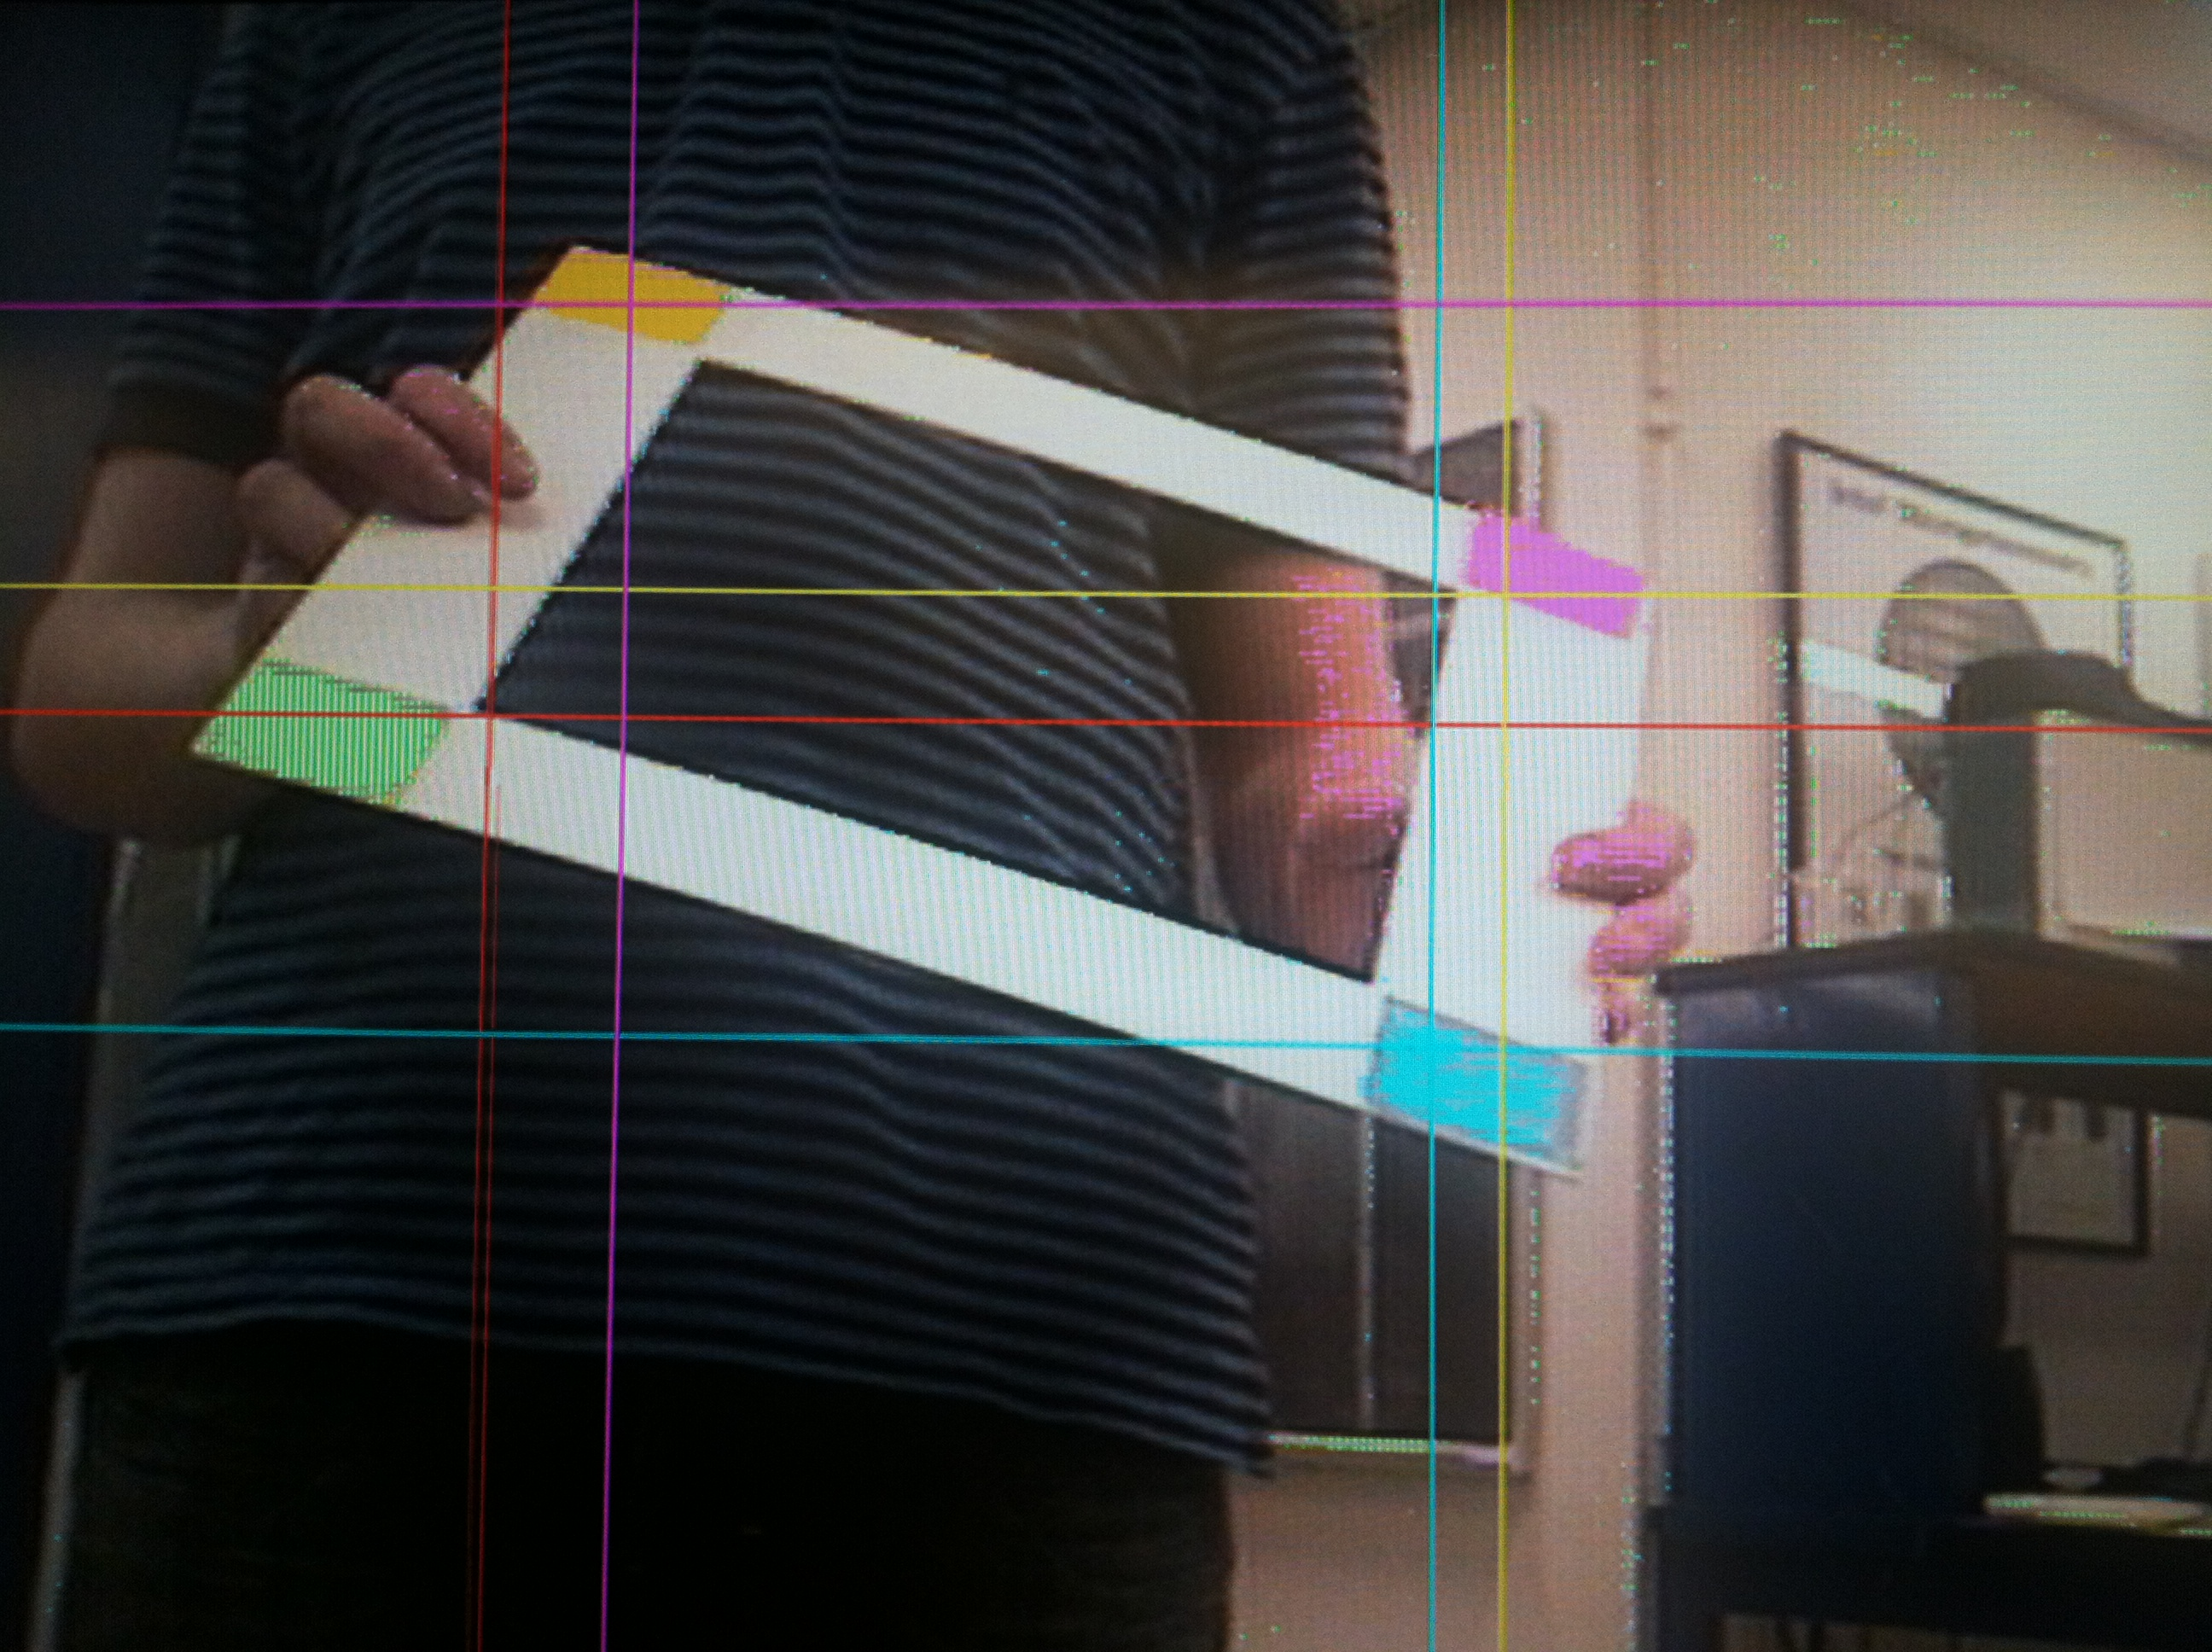
\includegraphics[width=0.75\textwidth]{images/IMG_0131.JPG}
\caption{\emph{Highlighting recognized colors, and displaying crosshairs on corners, so that color detection thresholds could be set more precisely.}}
\end{figure}

\subsection{Testing {\tt projective\_transform}}

To test {\tt projective\_transform}, a test jig was developed that provided the module with a list of input pixels, of linearly increasing luminance. The test jig also took the output of {\tt projective\_transform}, and saved it into an external file, along with the x and y coordinates of each output pixel. A MATLAB script was then used to display the results of {\tt projective\_transform}, along with the original image. The result of this MATLAB script is shown below. In this way, the algorithm used by {\tt projective\_transform} to distort the image was known to be correct.

\begin{figure}[h!]
\centering

\includegraphics[width=0.4\textwidth]{images/original.png}
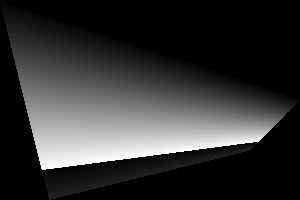
\includegraphics[width=0.4\textwidth]{images/output.png}
\caption{\emph{On the left, the sample input image used to test {\tt projective\_transform}. On the right, the output image from the testbench.}}
\end{figure}

However, this behavior simulation did not locate several problems that we had with setup and hold times on the signals that {\tt projective\_transform} transmits to {\tt memory\_interface}. In order to more easily diagnose these issues, we created a mode where {\tt lpf} sent a test pattern to {\tt projective\_transform} instead of real image data. With this mode enabled, it became very clear what the pattern of misplaced and miswritten pixels was.

\begin{figure}[h!]
\centering
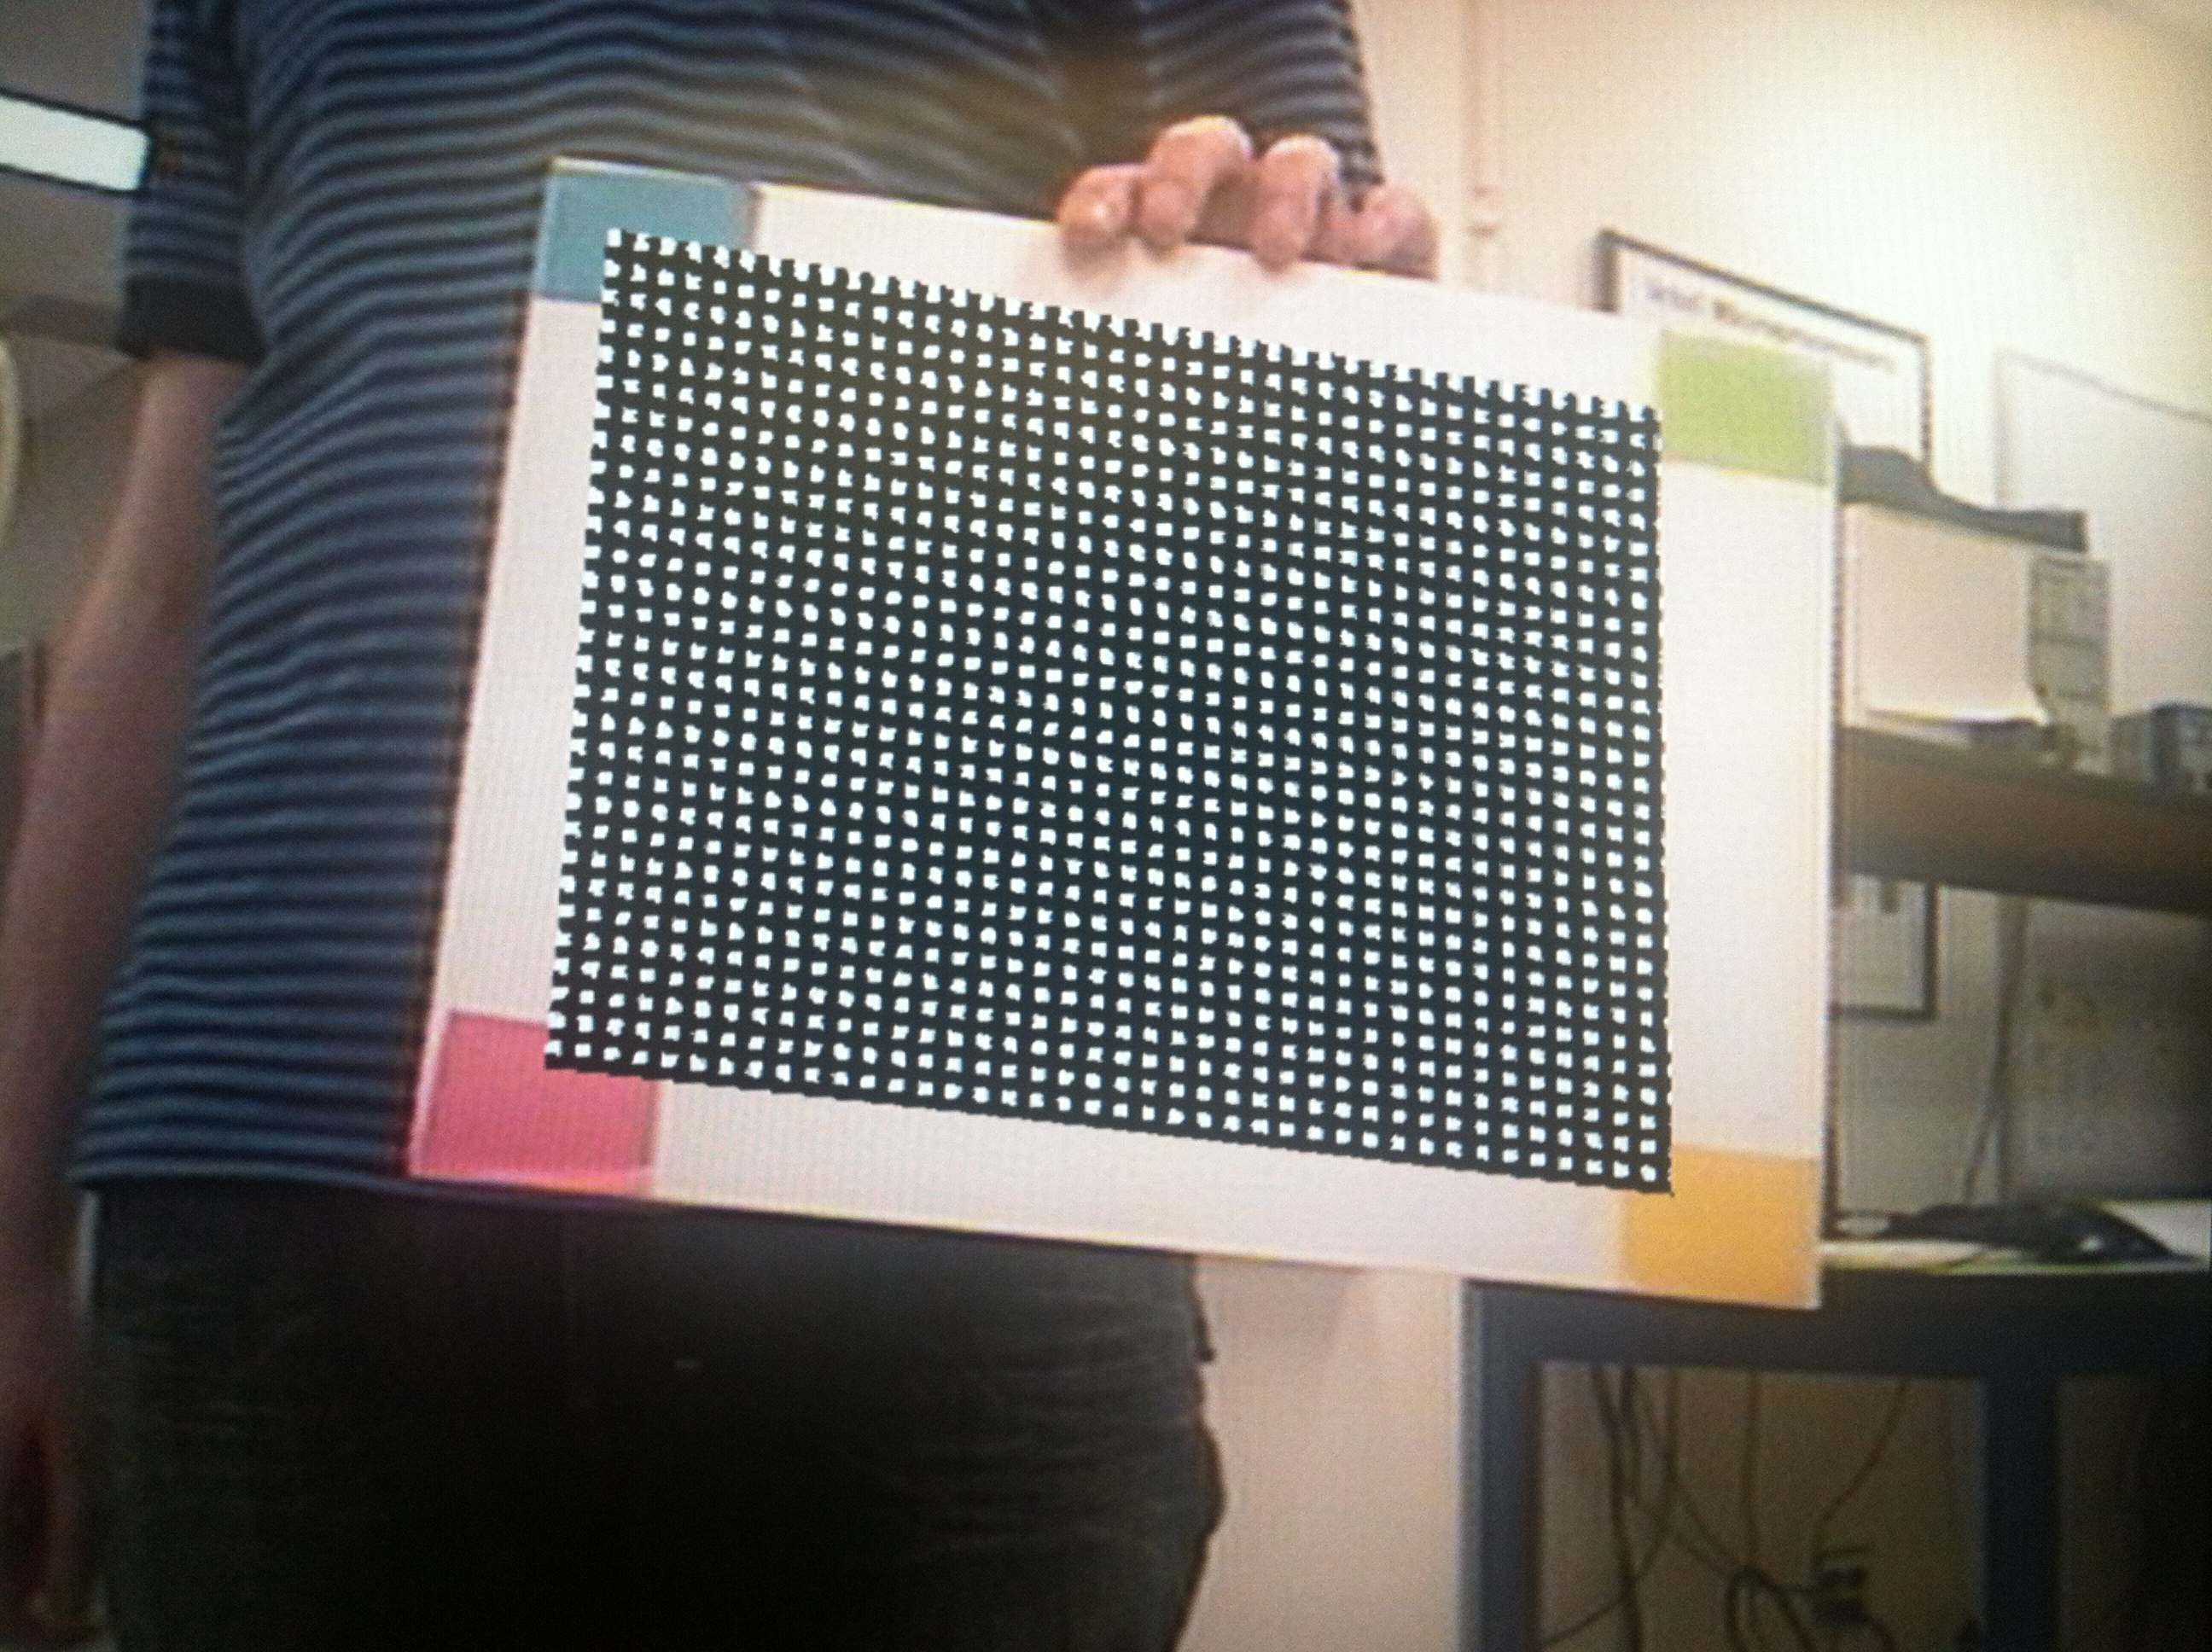
\includegraphics[width=0.75\textwidth]{images/IMG_0121.JPG}
\caption{\emph{Processing a test pattern instead of real image data, to decouple {\tt lpf} from {\tt memory\_interface}, and to make bugs in {\tt projecting\_transform} easier to recognize and diagnose.}}
\end{figure}

The logic analyzer also proved quite helpful for discovering these timing violations. However, we occasionally noticed that connecting a wire to the logic analyzer outputs was sufficient to change the behavior of the synthesized hardware, as it changed the synthesized routing path, and thus the routing delay. For this reason, using techniques such as the test pattern above for inferring the sources of bugs was necessary.

\subsection{Testing {\tt memory\_interface}}
{\tt memory\_interface} was tested in stages. Initially, this module was written and tested extensively using testbenches. The first testbench tested whether done flags pulsed two cycles after the request had been fed to the RAM. The second testbench tested whether priority was given to NTSC and VGA. The third testbench tested whether the switching of locations and blocks in memory was carried out effectively. Subsequent testbenches got progressively more complicated, combining several of these scenarios.

In lab, {\tt memory\_interface} was debugged by inputting test sequences into the RAM, placing requests on the (x,y) coordinates corresponding to the locations that were directly writtent to, and viewing the result on the logic analyzer. Once adequate functionality was ensured, this module was tested in conjunction with {\tt vga\_display} and {\tt ntsc\_capture}. Undesired behavior was seen in the output of {\tt memory\_interface} through {\tt vga\_display} until the clocks were synthesized correctly and the timing constraints were added to the constraints file. When the constraints were added, the ISE informed us of several critical pathways in {\tt memory\_interface}, which we then pipelined, resulting in a delay of four cycles, instead of the original two. However, this new {\tt memory\_interface} could now be run at frequencies much higher than the intended 50MHz.

A very sutble bug was introduced when we edited {\tt zbt\_6111} and changed it into {\tt zbt\_map}: When writing to the RAM, the data was being delayed by one clock cycle, instead of two. This problem manifested itself in very minor distortions in the video output, which we were able to ignore until the end of the development process. Once that typo was corrected, the pathway from {\tt ntsc\_capture} to {\tt vga\_display} was nearly perfect.

\subsection{Testing {\tt vga\_display}}
{\tt vga\_display} went through many iterations, as the needs and structure of the project changed. When we settled on using 25MHz and 50MHz clocks, the structure of {\tt vga\_display} matured to its current state. When we were considering clocks whose positive edges were not in phase, FIFOs were considered. However, writing a {\tt vga\_display} with two FIFOs proved to be very difficult, especially in guaranteeing constant throughput that is required by the video IC.

The {\tt xvga} module was not tested because it had been written and tested by 6.111 staff, and because all that needed to be changed was the bounds on the sync and blank regions, which are clearly defined for our resolution and refresh rate on \cite{xvga}. Initially, {\tt vga\_display} was tested with a test pattern fed directly into the {\tt vga\_display} module, based on flag requests and the {\tt hcount} and {\tt vcount} variables. Once this test pattern was displayed appropriately, we linked the module to {\tt memory\_interface}, which had been tested extensively at this point, and fed a test pattern through the RAM and into {\tt vga\_display}. When issues arose, we used the logic analyzer to discern what exactly was happening. Eventually, we linked up {\tt ntsc\_capture}, {\tt memory\_interface}, and {\tt vga\_display} and debugged what we saw on the logic analyzer. Color was added once the pathway from {\tt ntsc\_capture} to {\tt vga\_display} had stabilized. YCrCb to RGB conversion was implemented using lookup tables, and resulted in working color almost immediately after writing the LUTs.

\section{Conclusion}
% The conclusion of a project report typically summarizes the most important or innovative design features. The conclusion also often suggests ways in which the design could be improved. In your 6.111 report you should also make a point of summarizing the test results. If these were not fully satisfactory, they provide a natural basis for suggesting improvements. As a guide to others, it is very helpful to include some discussion of the problems you met in your initial design and what you did to overcome these problems. 

The Augmented Reality Image Processing System used digital logic to scale, skew, rotate, and translate a video image to specific coordinates in real time. It was also able to precisely locate the corners of a frame in the image by looking for specific hues. While we did not have time to implement the planned low pass filter, the output of {\tt augreal} was already of an acceptably high quality.

Possible improvements include adding the aforementioned low pass filter, allowing arbitrary image files to be displayed, and improving object recognition to use algorithms that do not rely on hue markers. However, because {\tt augreal} already has a very high throughput of 79 MiB of data per second, and a relatively fast clock frequency of 50 Mhz, adding these modification would require extending the length of the image processing pipeline beyond four frame buffers, which would require additional RAM hardware.

Overall, we were very pleased with the smoothness of the frame rate, the reliability of the corner recognition, the success of our use of ZBT memory, the appearance of the image projection, and the overall ``wow'' and ``fun'' of the system.

\begin{thebibliography}{9}

\bibitem{restoring}
  Malek, Miroslaw.
  2002.
  \emph{Division algorithms.}
  Available: \\ \url{http://devel-rok.informatik.hu-berlin.de/svn/TI2/2006/folien/pdf/eng\_ca12.pdf}

\bibitem{xvga}
  Ickes, Nathan.
  2007.
  \emph{VGA Video Output}
  \url{http://www-mtl.mit.edu/Courses/6.111/labkit/vga.shtml}

\bibitem{ycrcb}
  Pillai, Latha.
  2001.
  \emph{XAPP283: Color Space Converter}
  \url{http://www-mtl.mit.edu/Courses/6.111/labkit/appnotes/xapp283.pdf}

\end{thebibliography}

\newpage
\appendix
\section{Project Source Code}
\subsection{{\tt labkit.v}}

\lstinputlisting{../../src/augreal/labkit.v}
	  	
\subsection{{\tt ntsc\_capture.v}}
	  	
\lstinputlisting{../../src/augreal/ntsc_capture.v}
\subsection{{\tt memory\_interface.}}
	  	
\lstinputlisting{../../src/augreal/memory_interface.v}
	  	
\subsection{{\tt object\_recognition.v}}
	  	
\lstinputlisting{../../src/augreal/object_recognition.v}

\subsection{{\tt test\_object\_recognition.v}}

\lstinputlisting{../../src/test_object_recognition.v}
	  	
\subsection{{\tt lpf.v}}
	  	
\lstinputlisting{../../src/augreal/lpf.v}
	  	
\subsection{{\tt projective\_transform.v}}
	  	
\lstinputlisting{../../src/augreal/projective_transform_srl.v}

\subsection{{\tt projective\_transform\_testbench.v}}

\lstinputlisting{../../src/test_projective_transform/test_projective_transform/projective_transform_testbench.v}
	  	
\subsection{{\tt divider.v}}
	  	
\lstinputlisting{../../src/augreal/divider.v}
	  	
\subsection{{\tt clock\_gen.v}}
\lstinputlisting{../../src/augreal/clock_gen.v}
	  	
\subsection{{\tt vga\_write.v}}
	  	
\lstinputlisting{../../src/augreal/vga_write_new.v}
	  	
\subsection{{\tt ycbcr2rgb.v}}
	  	
\lstinputlisting{../../src/augreal/ycbcr2rgb.v}
	  	
\subsection{{\tt parameter\_set.v}}	  	
\lstinputlisting{../../src/augreal/parameter_set.v}
\subsection{{\tt params.v}}	  	
\lstinputlisting{../../src/augreal/params.v}	  	
\subsection{{\tt zbt\_test\_pattern.v}}  	
\lstinputlisting{../../src/augreal/zbt_test_pattern.v}

\end{document}
